\newpage
\section{Ejemplos y resultados}

\subsection{C�digos correctos y resultados generados}
\subsubsection{Primer ejemplo: Par�bola}

\lstset{language=C}
\begin{lstlisting}
function id(x)
  return x

plot (id(x), id(x * x)) for x = -10 .. 0.5 .. 10
\end{lstlisting}

Este ejemplo simple define la funci�n identidad y en base a eso ploteamos una par�bola cuadr�tica con X entre -10 y 10. Cabe destacar que si bien el ejemplo parece trivial, hace uso de una de las particularidades del lenguaje que es la de definir funciones con cuerpos sin llaves cuando hay una sola instrucci�n.
\newline

El ejemplo devuelve los siguientes puntos esperados:
\newline

-10 100

-9.5 90.25

-9 81

-8.5 72.25

...

9.5 90.25

10 100
\newline

A su vez graficados obtenemos:

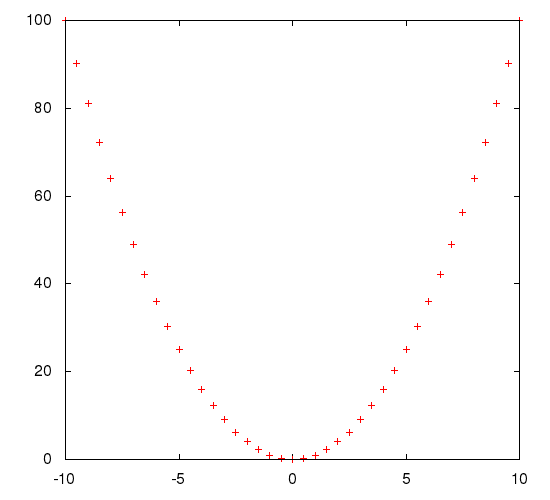
\includegraphics[trim = -20mm 0mm 0mm 0mm, scale=0.8]{img/parabola.png}
\newpage

\subsubsection{Segundo ejemplo: Seno}
\noindent \begin{lstlisting}
function fact(n) {
  if n < 2 then
    return 1
  i = 1
  while n > 0 {
    i = i * n
    n = n - 1
  }
  return i
}

function sin(x) {
  x2 = x * x
  res = 0
  power_x = x
  sign = 1
  i = 0
  while i < 30 {
    res = res + sign * power_x / fact(2 * i + 1)
    power_x = power_x * x2
    sign = - sign
    i = i + 1
  }
  return res
}

function id(x)
  return x

plot (id(x), sin(x)) for x=0..0.1..2*pi
\end{lstlisting}

Este segundo ejemplo nos deja ver algunas funcionalidades m�s complejas del lenguaje como las estructuras de control while e if. Podemos observar tambi�n que ocurren llamados entre funciones ya que \emph{sin} llama a \emph{fact}. Tambi�n se observan asignaciones y operaciones aritm�ticas m�s complejas. Por �ltimo, vemos que se puede llamar a la constante \emph{pi}. Cabe destacar que en este ejemplo hay bloques de instrucciones con y sin llaves en el mismo c�digo.
\newline

El ejemplo devuelve los siguientes puntos esperados:
\newline

-0.1 0.0998334

-0.2 0.198669

-0.3 0.29552

...

6.2 -0.0830894
\newpage

A su vez graficados obtenemos la sinusoide esperada:

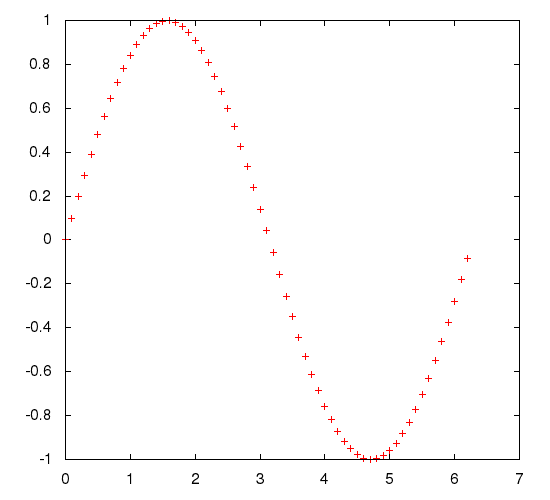
\includegraphics[trim = -20mm 0mm 0mm 0mm, scale=0.8]{img/seno.png}

\subsubsection{Tercer ejemplo: Superficie 3D!}

\begin{lstlisting}
function fact(n) {
  if n < 2 then
    return 1
  i = 1
  while n > 0 {
    i = i * n
    n = n - 1
  }
  return i
}

function sin(x) {
  while x > 2 * pi {
    x = x - 2 * pi
  }
  x2 = x * x
  res = 0
  power_x = x
  sign = 1
  i = 0
  while i < 30 {
    res = res + sign * power_x / fact(2 * i + 1)
    power_x = power_x * x2
    sign = - sign
    i = i + 1
  }
  return res
}

function cos(x) {
  while x > 2 * pi {
    x = x - 2 * pi
  }
  x2 = x * x
  res = 0
  power_x = 1
  sign = 1
  i = 0
  while i < 30 {
    res = res + sign * power_x / fact(2 * i)
    power_x = power_x * x2
    sign = - sign
    i = i + 1
  }
  return res
}

plot (cos(1 * t) - cos(200 * t) ^ 3, sin(200 * t) - sin(2 * t) ^ 4)
for t = 0..0.001..2*pi
\end{lstlisting}

Este tercer ejemplo adem�s de ser el m�s intrincado de los tres propuestos, hace uso de otras dos funcionalidades no vistas en los anteriores. Primero una menor que es la de un \emph{if} con \emph{then} y un bloque de una sola instrucci�n. Luego, el uso del comando plot con una instrucci�n en lugar de una funci�n. Como vemos, ambos argumentos de la funci�n plot no son llamados a funciones, sino instrucciones con operaciones aritm�ticas que a su vez llaman funciones. Esta es una de las modificaciones que propusimos al lenguaje pedido en el enunciado. Si hubi�ramos querido hacer
\begin{lstlisting}
cos(1 * t) - cos(200 * t) ^ 3
\end{lstlisting}
tendr�amos que haber hecho una funci�n que hiciera eso y llamarla desde plot. En su lugar, la modificaci�n permite hacerlo inline.
\newpage

No presentamos los puntos ya que no son de una funci�n conocida y por lo tanto no es simple encontrarle la l�gica. Sin embargo, obtenemos el siguiente plot esperado:
\newline
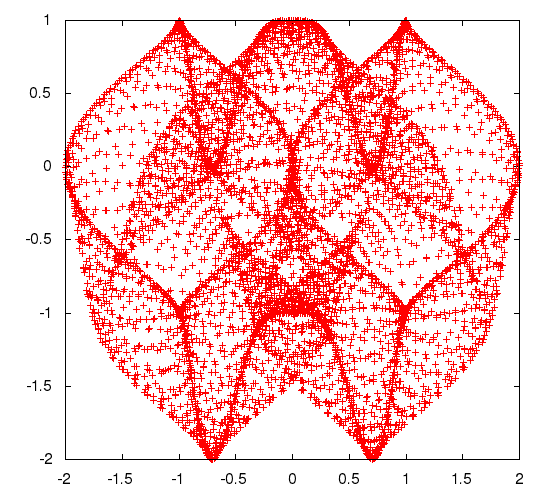
\includegraphics[trim = -20mm 0mm 0mm 0mm, scale=0.8]{img/rara.png}

\subsection{C�digos con errores}
\subsubsection{Primer ejemplo}
\subsubsection{Segundo ejemplo}
\subsubsection{Tercer ejemplo}